%!TEX root = ..\..\main.tex

\section{Diskussion}
\label{sec:Auswertung}
Nach der radialen Entzerrung mit dem implementierten Verfahren kommt man zu dem in Abbildung~\ref{fig:Ergebnis} und Abbildung~\ref{fig:diffsResult} gezeigten Ergebnis. Die Koeffizienten der radialen Entzerrung sind für dieses Resultat in Gleichung~\ref{equ:radial_koeff} notiert. 

\begin{align}
a &=  2.8974105705613364E-8 \nonumber \\
b &= -4.0458117860182954E-15 \nonumber \\
c &=  2.8527492714683317E-21
\label{equ:radial_koeff}
\end{align}

\begin{figure}
	\subfigure{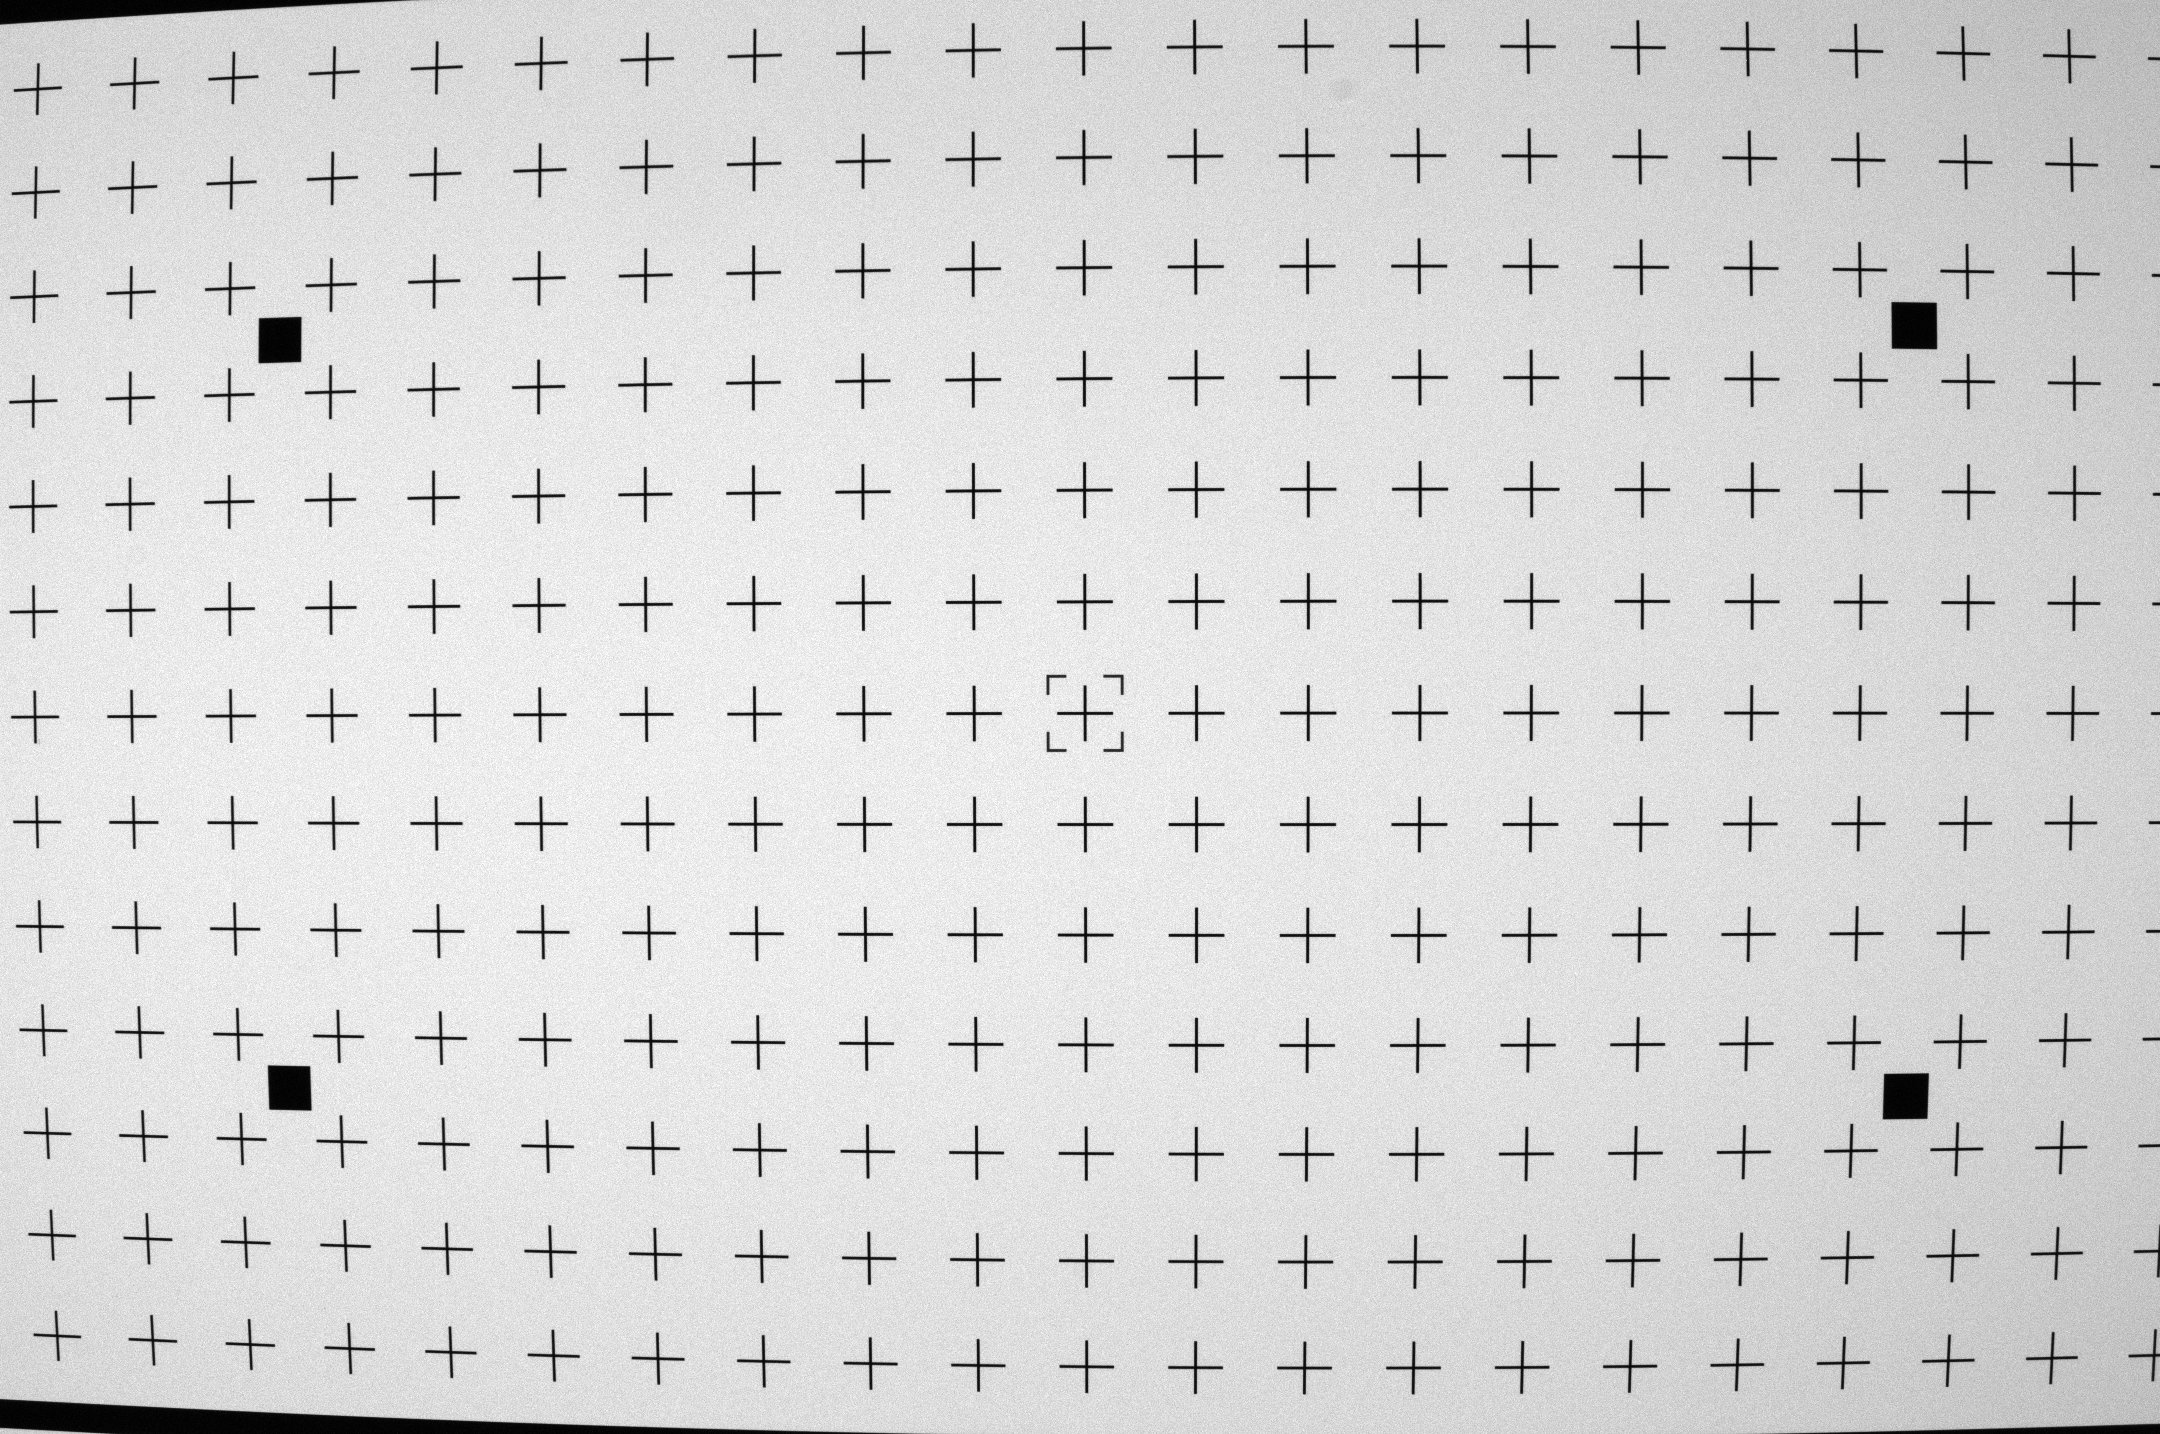
\includegraphics[width=\textwidth/2]{Images/Auswertung/Testbild1/18mm_11-1.jpg}}
	\subfigure {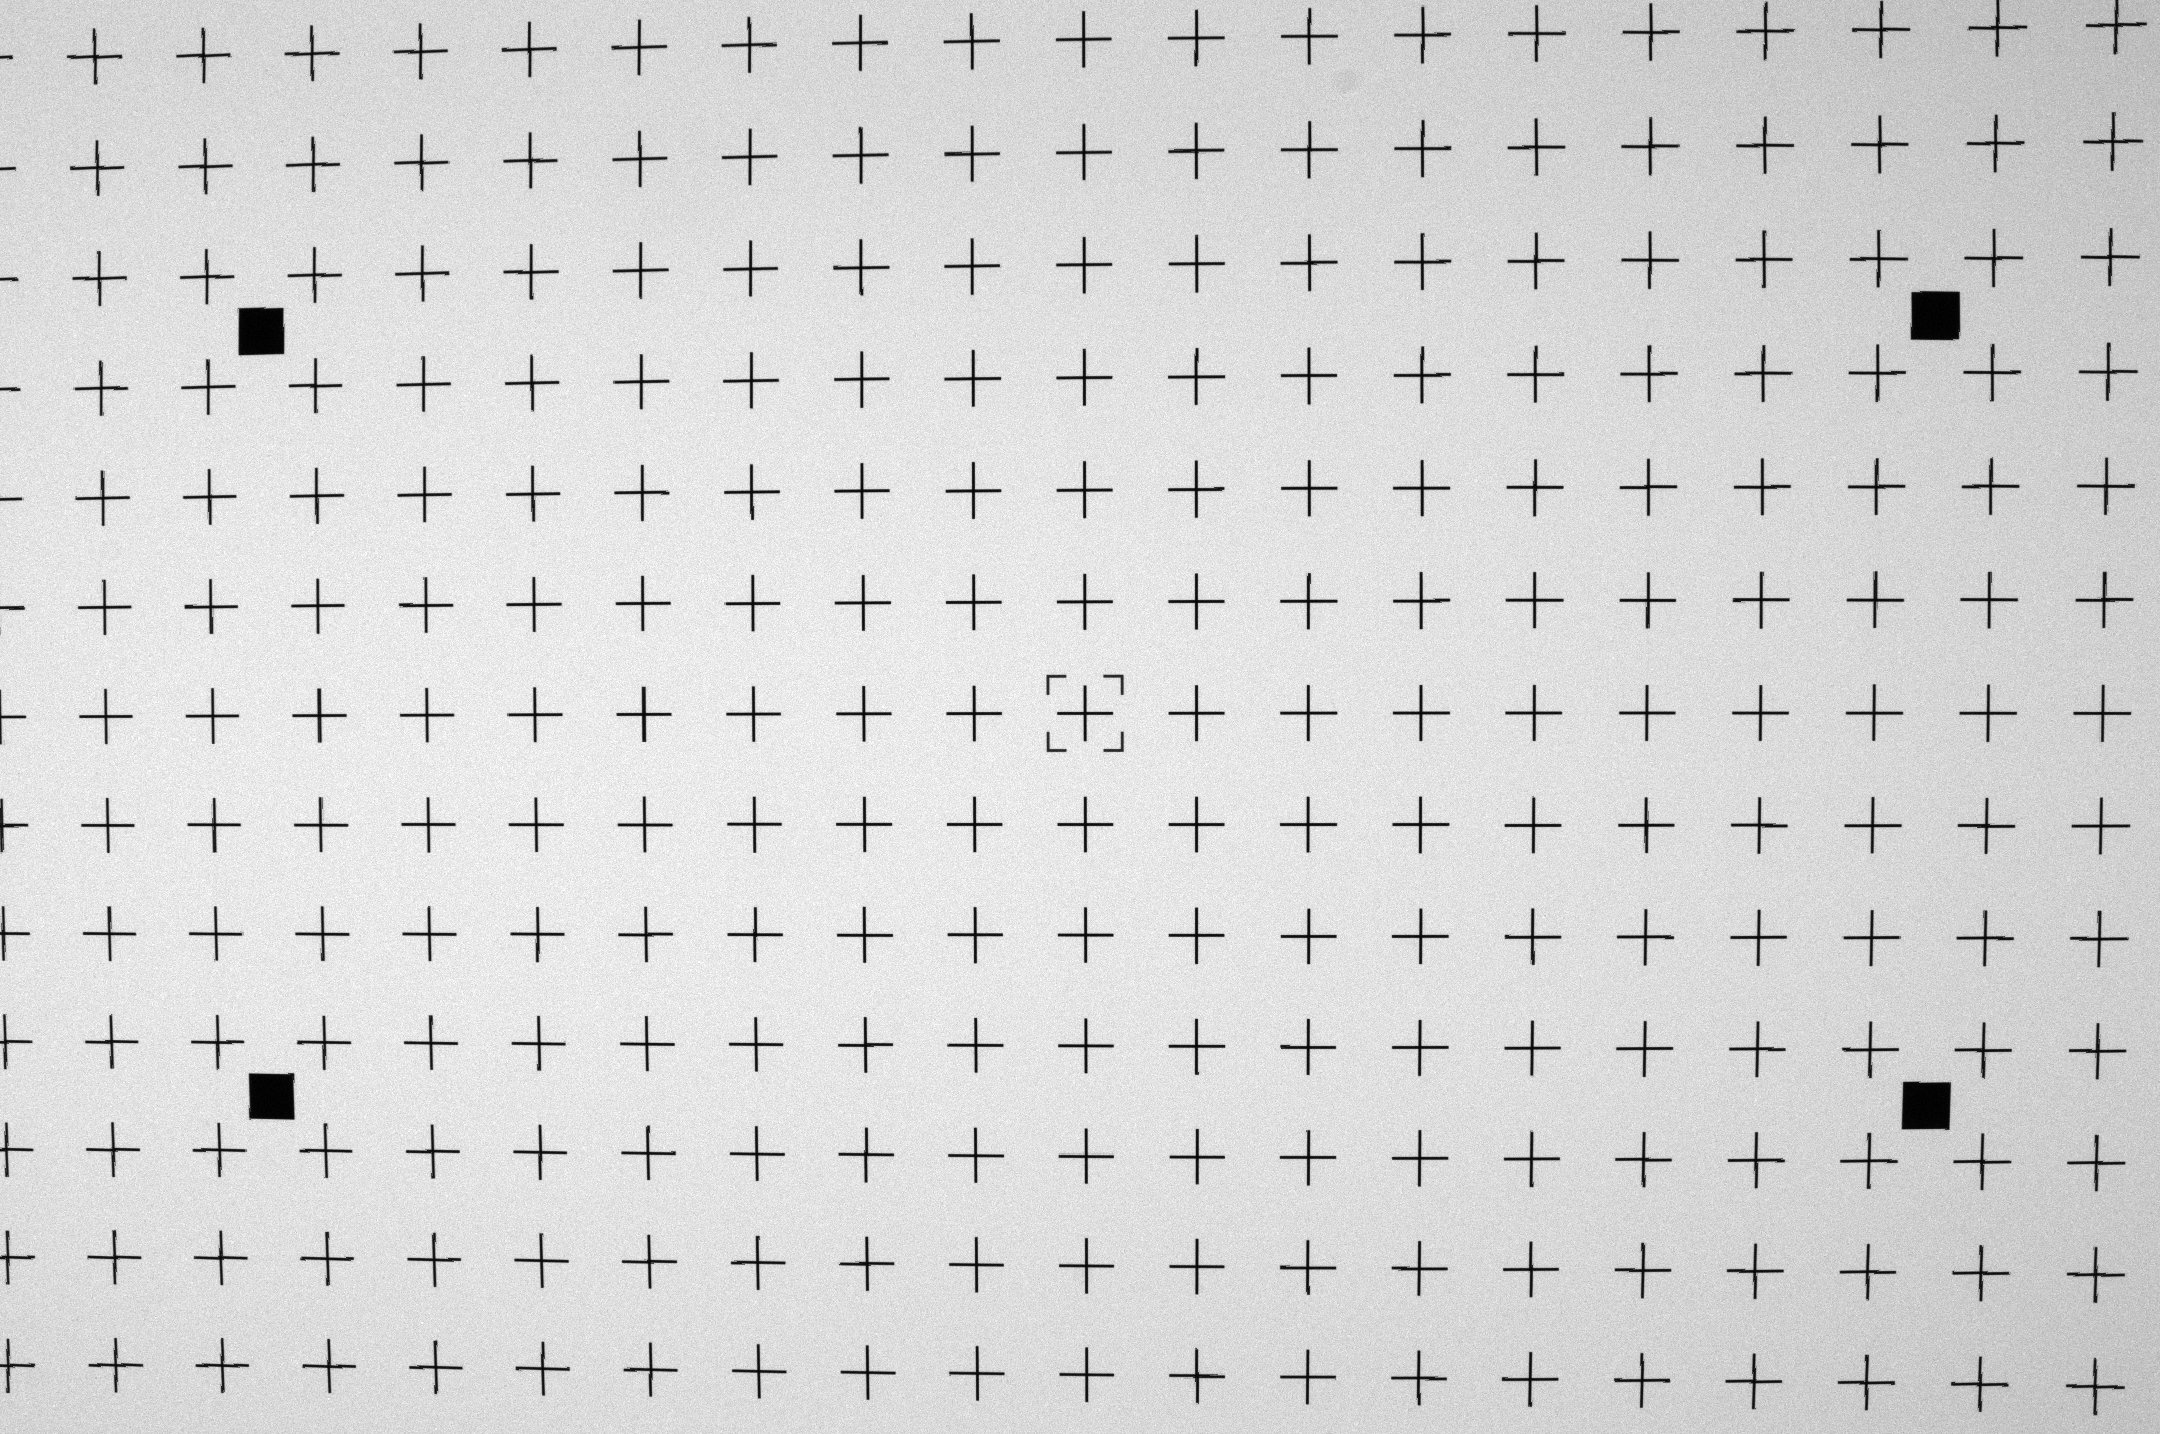
\includegraphics[width=\textwidth/2]{Images/Auswertung/Testbild1/Radial.jpg}}
	\caption{Links: Ausgangsbild. Rechts: Resultat der Radialen Entzerrung}
	\label{fig:Ergebnis}
\end{figure}
	
Anhand der Abbildung~\ref{fig:Ergebnis} ist deutlich zu erkennen, dass das Gitter gleichmäßiger und gerader wird. Des Weiteren wird durch Abbildung~\ref{fig:diffsResult} verdeutlicht, dass sich die Differenzen zwischen Start- und Zielkoordinaten der Punkte verkleinern. Dies bestätigt, dass das Verfahren funktioniert.

\begin{figure}
	\subfigure {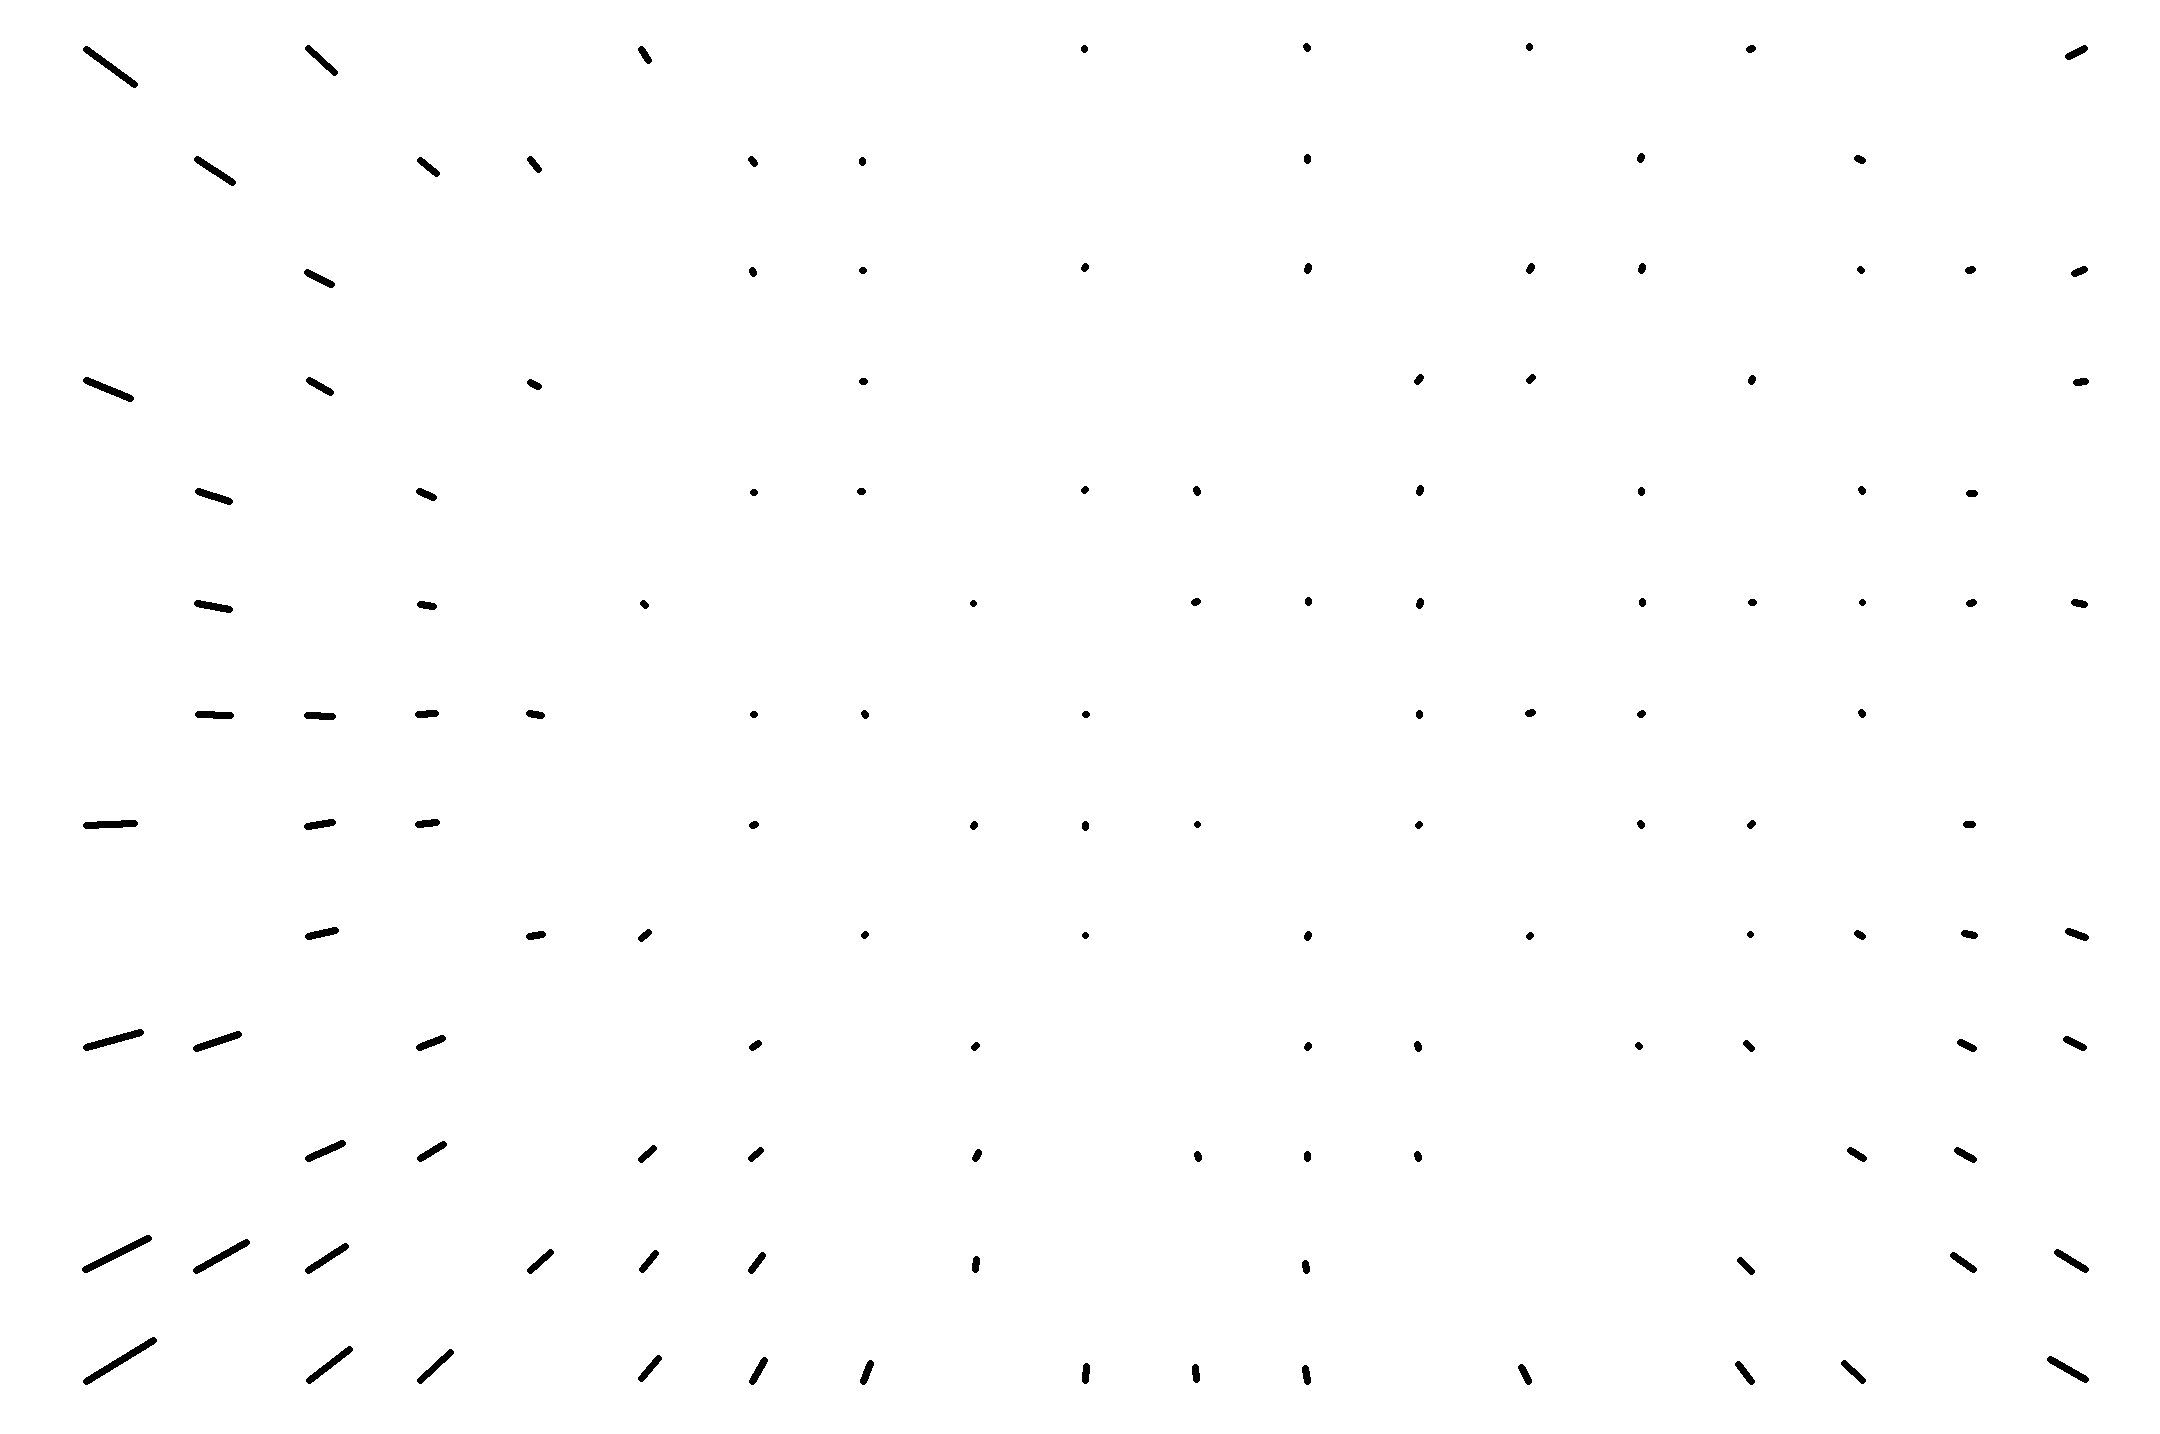
\includegraphics[width=\textwidth/2]{Images/Auswertung/Testbild1/SourceImage with PointPairs_onlydiffs.jpg}}
	\subfigure{	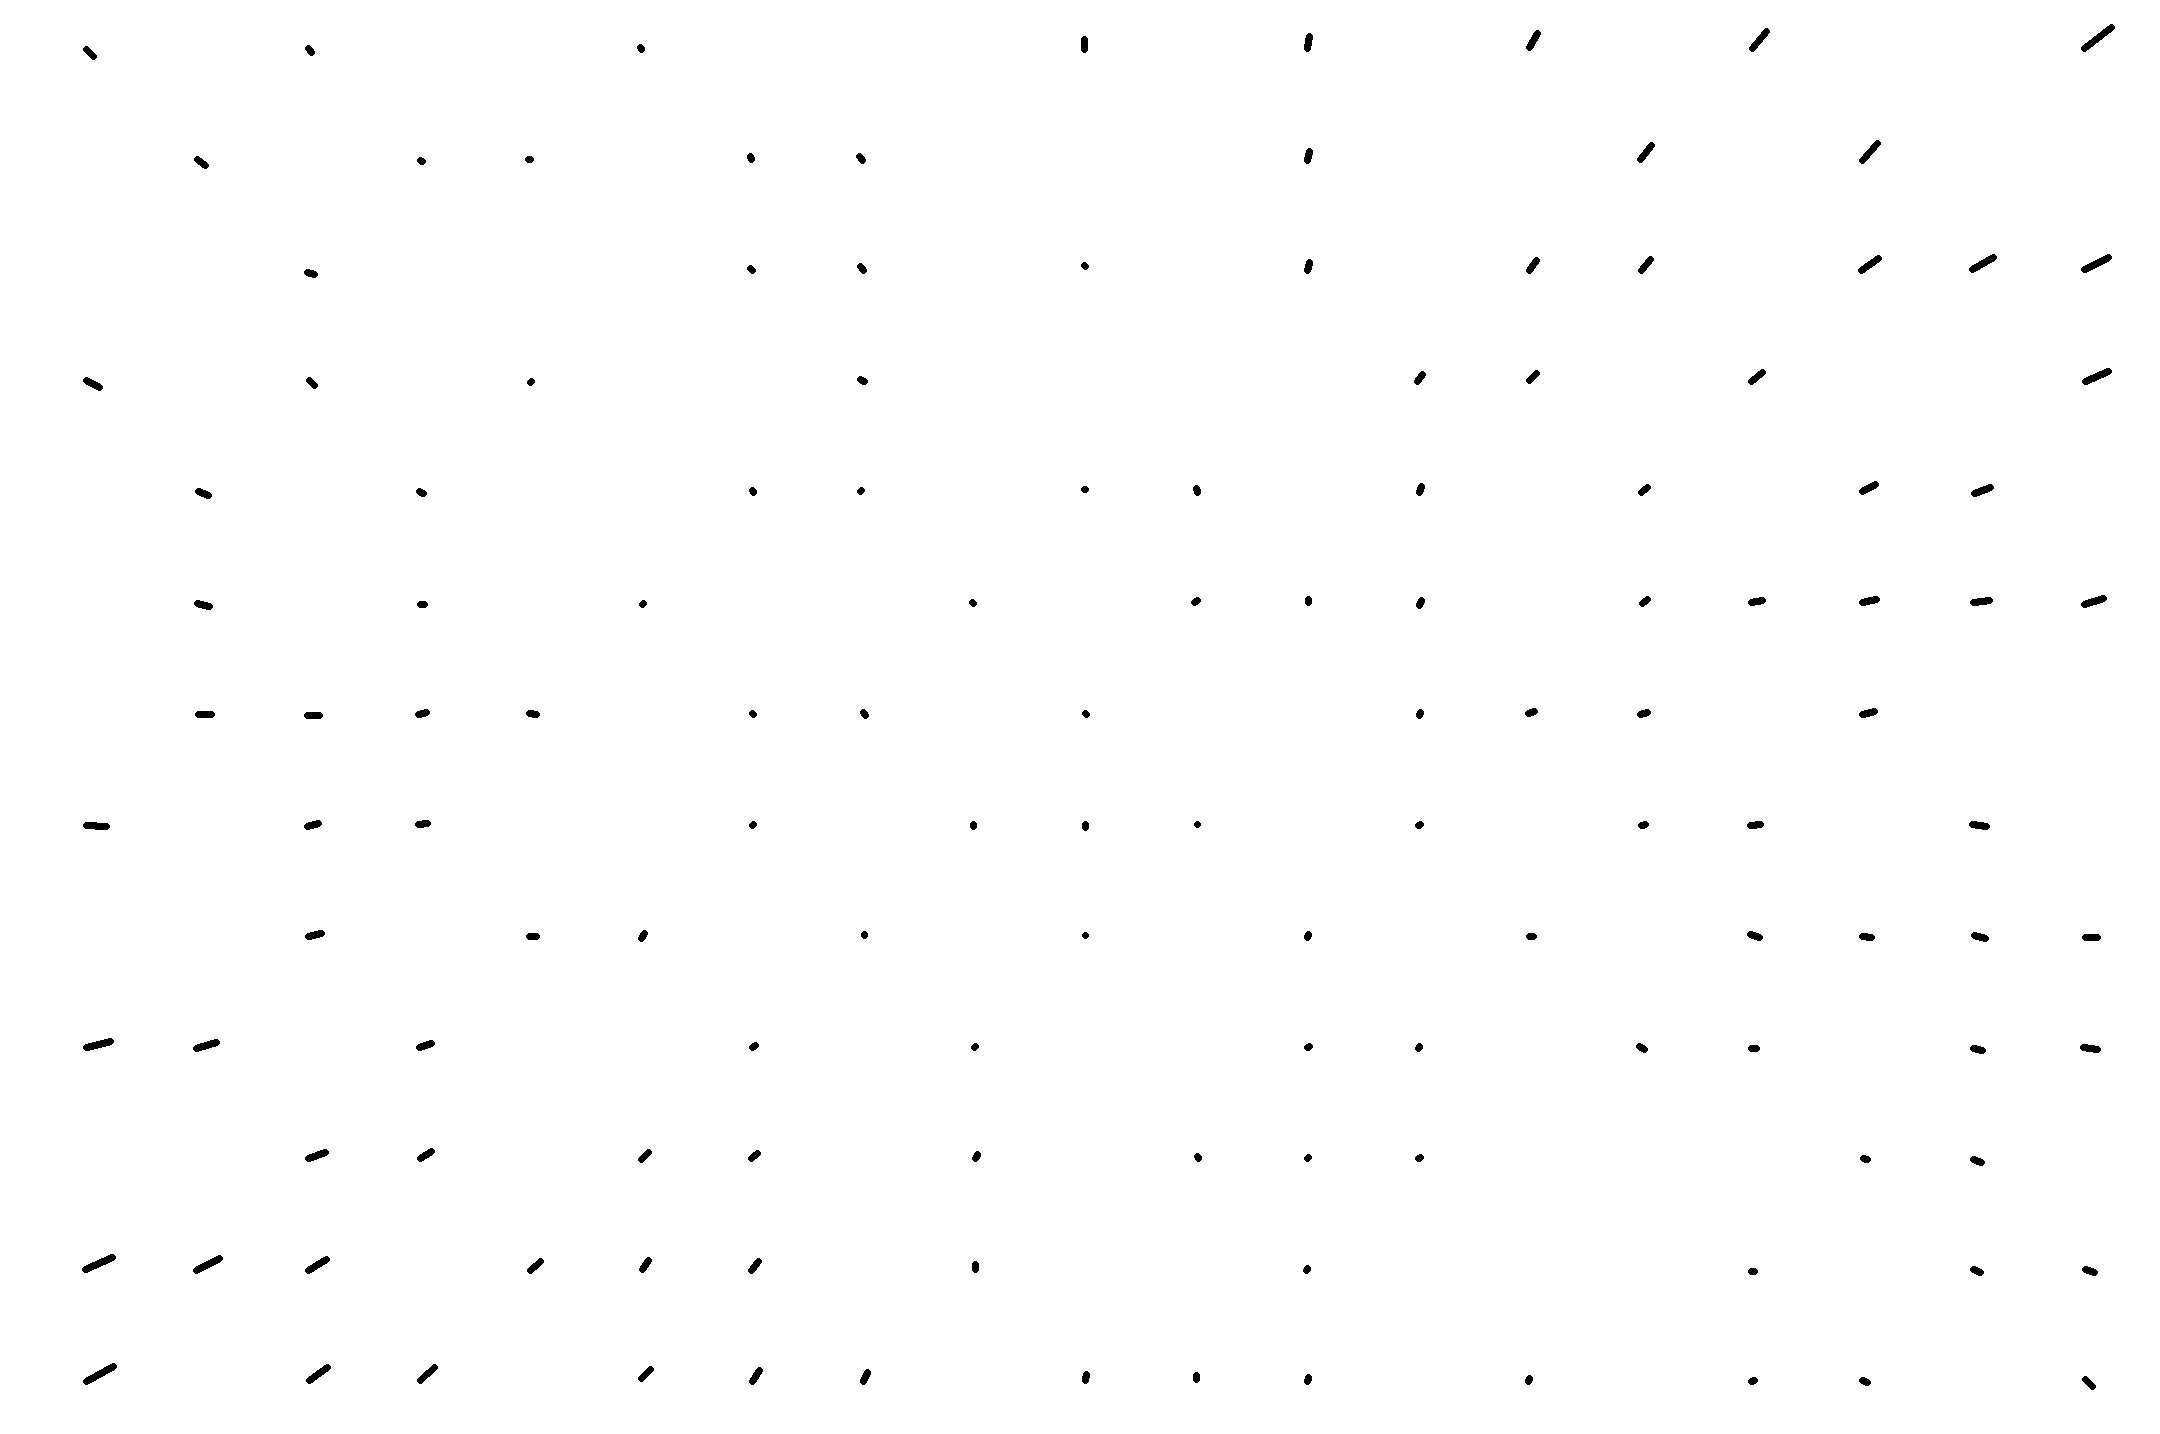
\includegraphics[width=\textwidth/2]{Images/Auswertung/Testbild1/Radial_onlydiffs.jpg}}
	\caption{Links: Differenzen zwischen den idealen und realen Stützpunkten. \\Rechts: Differenzen zwischen den idealen und transformierten Stützpunkten.}
	\label{fig:diffsResult}
\end{figure}

Bei genauer Betrachtung der Differenzen in Abbildung~\ref{fig:diffsResult} ist jedoch zu erkennen, dass sich auf der Diagonalen ausgehend von der linken oberen Ecke die Differenzen deutlich verkleinern und nahezu mit den idealen Koordinaten übereinstimmen. Während sie auf der anderen Diagonalen rechten Bereich zwar verkleinern, aber noch signifikante Differenzen sichtbar sind. Dies ist auf die perspektivische Verzerrung zurückzuführen, welche entsteht wenn die Kamera nicht exakt entlang der optischen Achse ausgerichtet ist. Die Folge sind ungleiche Abstände der Punkte auf beiden Seiten, wie in Abbildung~\ref{fig:diffsResult} zu erkennen ist. Da das Modell der RDF aber ausgehend vom Bildzentrum konstant zunehmende Abstände annimmt, kommt es zu der leicht ungenauen Korrektur der radialen Verzerrung.
Es existiert somit eine zusätzliche perspektivische Verzerrung für die eine vorherige projektive Transformation notwendig ist damit das implementierte Verfahren erfolgreich angewendet werden kann.

Weiterhin ist für das Verfahren problematisch, wenn die Verzerrung sehr stark ist oder im mittleren Radius größer ist als im äußeren Radius (Fish-Eye-Effekt)\cite{WangRaddist}. Bei diesem Effekt sind aber die äußeren Start und Ziel-Koordinaten sehr dicht beieinander und dies wird vom  Optimierer berücksichtigt mit der Folge, dass die korrespondierenden Bildbereiche nur gering korrigiert werden. Für diesen Effekt ist das Modell aus Gleichung~\ref{equ:RDF} nicht die optimale Lösung und es muss auf komplexere Modelle zurückgegriffen werden~\cite{WangRaddist}. 

Ein zusätzlicher Nachteil der Implementierung ist die manuelle Generierung der Punktpaare mit UnwrapJ. Bei der manuellen Positionierung der Koordinaten-Paare können unter Umständen größere Messfehler für die Abstände einzelner Paare auftreten und die Abstände geringer ausfallen als dies erwartet wird. So können für die entsprechenden Bildbereiche ein fehlerhafter Korrekturfaktor angenähert werden und im resultierenden Bild können stellenweisen deutliche gebogene Linien ausgemacht werden. 

